\documentclass[hyperref,]{ctexart}
\usepackage{lmodern}
\usepackage{amssymb,amsmath}
\usepackage{ifxetex,ifluatex}
\usepackage{fixltx2e} % provides \textsubscript
\ifnum 0\ifxetex 1\fi\ifluatex 1\fi=0 % if pdftex
  \usepackage[T1]{fontenc}
  \usepackage[utf8]{inputenc}
\else % if luatex or xelatex
  \ifxetex
    \usepackage{xltxtra,xunicode}
  \else
    \usepackage{fontspec}
  \fi
  \defaultfontfeatures{Mapping=tex-text,Scale=MatchLowercase}
  \newcommand{\euro}{€}
\fi
% use upquote if available, for straight quotes in verbatim environments
\IfFileExists{upquote.sty}{\usepackage{upquote}}{}
% use microtype if available
\IfFileExists{microtype.sty}{%
\usepackage{microtype}
\UseMicrotypeSet[protrusion]{basicmath} % disable protrusion for tt fonts
}{}
\ifxetex
  \usepackage[setpagesize=false, % page size defined by xetex
              unicode=false, % unicode breaks when used with xetex
              xetex]{hyperref}
\else
  \usepackage[unicode=true]{hyperref}
\fi
\usepackage[usenames,dvipsnames]{color}
\hypersetup{breaklinks=true,
            bookmarks=true,
            pdfauthor={蓝海; 彭莉},
            pdftitle={PB-ROE:技术报告},
            colorlinks=true,
            citecolor=blue,
            urlcolor=blue,
            linkcolor=magenta,
            pdfborder={0 0 0}}
\urlstyle{same}  % don't use monospace font for urls
\usepackage{graphicx,grffile}
\makeatletter
\def\maxwidth{\ifdim\Gin@nat@width>\linewidth\linewidth\else\Gin@nat@width\fi}
\def\maxheight{\ifdim\Gin@nat@height>\textheight\textheight\else\Gin@nat@height\fi}
\makeatother
% Scale images if necessary, so that they will not overflow the page
% margins by default, and it is still possible to overwrite the defaults
% using explicit options in \includegraphics[width, height, ...]{}
\setkeys{Gin}{width=\maxwidth,height=\maxheight,keepaspectratio}
\setlength{\emergencystretch}{3em}  % prevent overfull lines
\providecommand{\tightlist}{%
  \setlength{\itemsep}{0pt}\setlength{\parskip}{0pt}}
\setcounter{secnumdepth}{5}

\title{PB-ROE:技术报告}
\author{蓝海 \and 彭莉}
\date{}

% Redefines (sub)paragraphs to behave more like sections
\ifx\paragraph\undefined\else
\let\oldparagraph\paragraph
\renewcommand{\paragraph}[1]{\oldparagraph{#1}\mbox{}}
\fi
\ifx\subparagraph\undefined\else
\let\oldsubparagraph\subparagraph
\renewcommand{\subparagraph}[1]{\oldsubparagraph{#1}\mbox{}}
\fi

\begin{document}
\maketitle

{
\setcounter{tocdepth}{2}
\tableofcontents
}
\section{PB和ROE}\label{pbroe}

\subsection{PB的历史演进}\label{pb}

PB勾结了股票市场上的两个信号:

\begin{itemize}
\tightlist
\item
  Price(价格):这是个在市场上只要交易就变化着的快信号;
\item
  Book
  (会计价值):这是由会计师一定的会计准则为投资者记录的企业的账面价值,它是由企业的历史活动累积的、会计师周期性更新的慢信号。
\end{itemize}

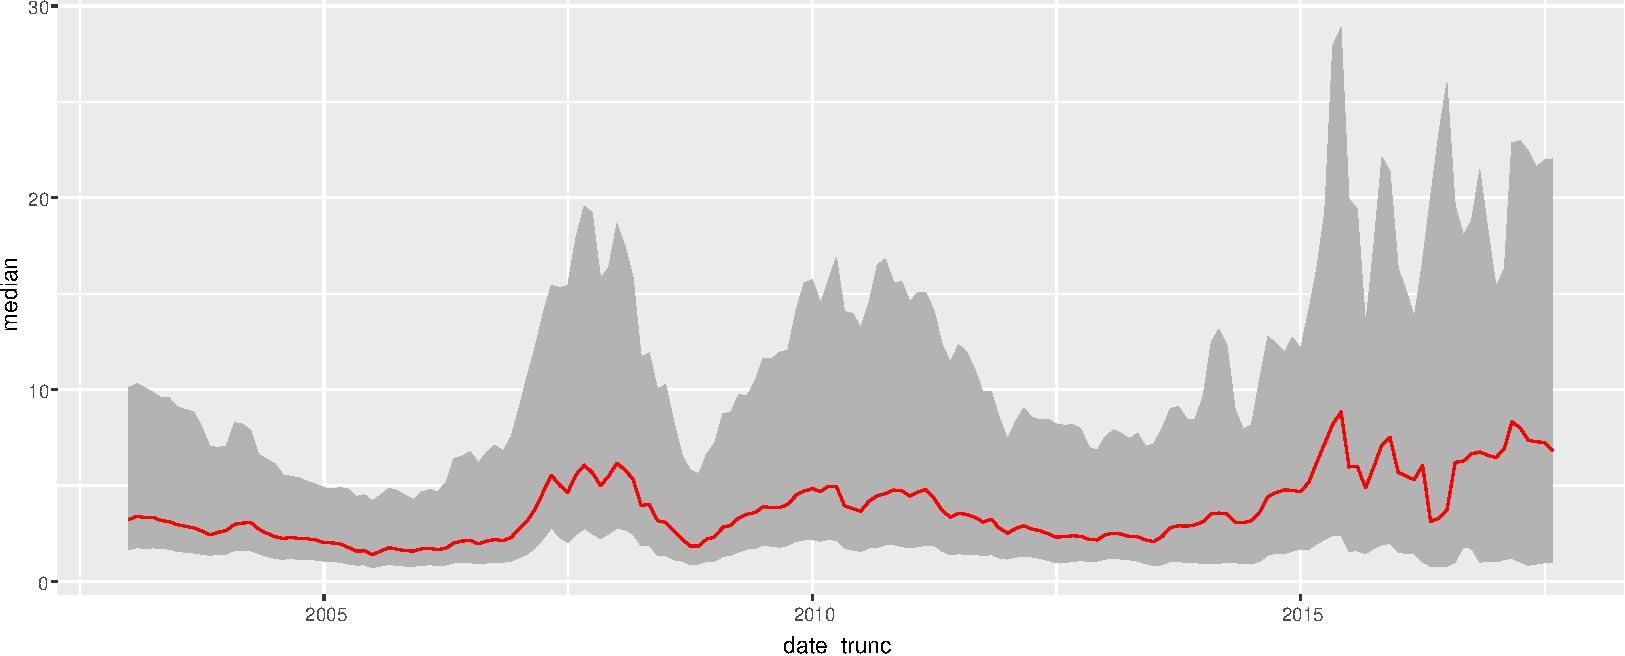
\includegraphics{PB-ROE_files/figure-latex/unnamed-chunk-2-1.pdf}
阴影部分是同期市场上所有股票一月之间的PB值的5\%至95\%。而红色的线则代表这些PB数值的中位数。不难理解2007年和2015年市场泡沫期间,市场对于股票价格整个的高估,表现在PB值无论是低5\%、高的95\%还是中位数都整体上扬,伴随市场指数攀顶而到达顶点。有意思的是,这种估值泡沫往往在随后的市场恢复中接着出现,尽管指数恢复的情况远未能达到前期泡沫时水平,但是PB值却十分接近泡沫时的高点。

以上现象可以用股票价格的恢复来解释吗? 我们看同一时期,沪深300的形态是:

\begin{figure}[htbp]
\centering
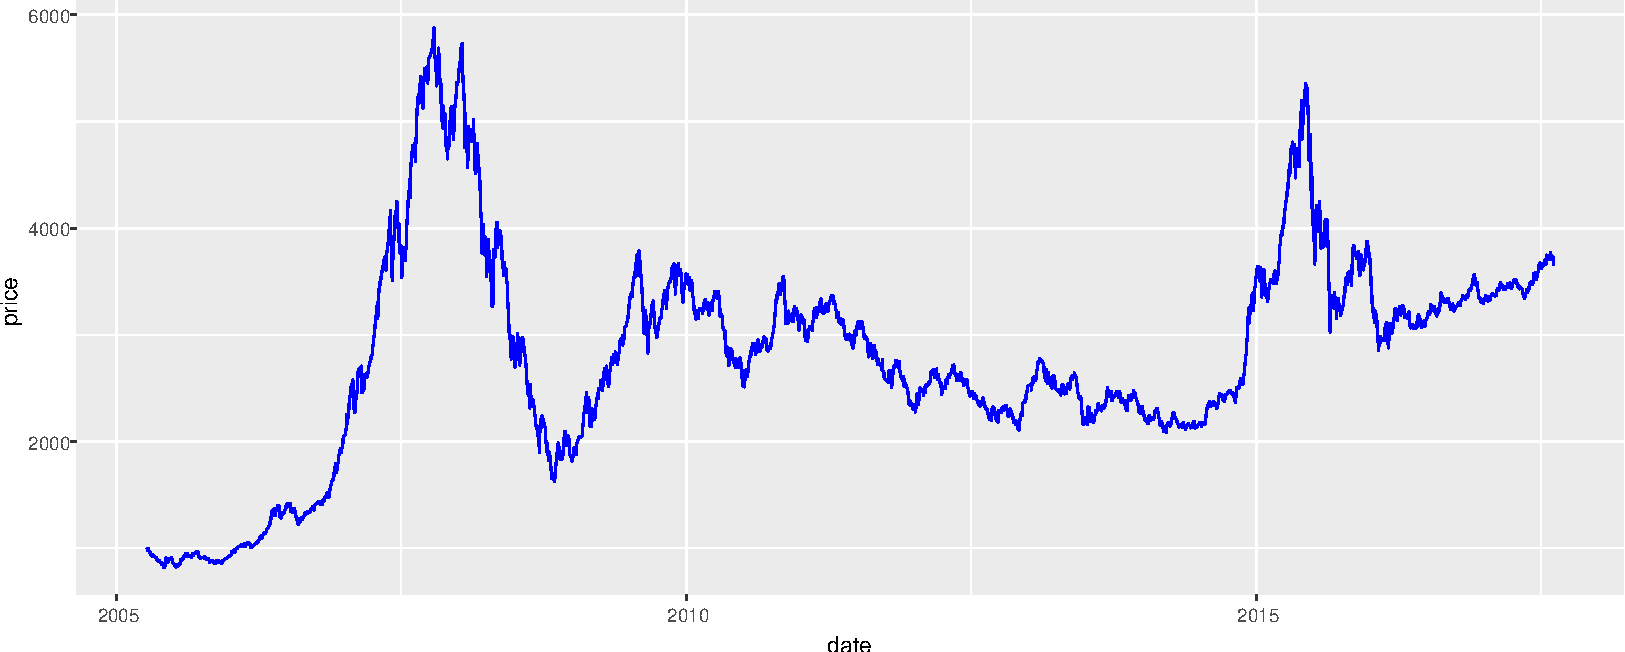
\includegraphics{PB-ROE_files/figure-latex/unnamed-chunk-3-1.pdf}
\caption{沪深300历史趋势}
\end{figure}

显然,股票价格是能够部分解释PB的上扬,但是不能解释为什么会恢复的远远超出价格恢复的幅度,而几乎接近泡沫时期的高点。那么是由于账目价值恶化的结果吗?

同一时期,上市公司账目价值的变化是:

\begin{figure}[htbp]
\centering
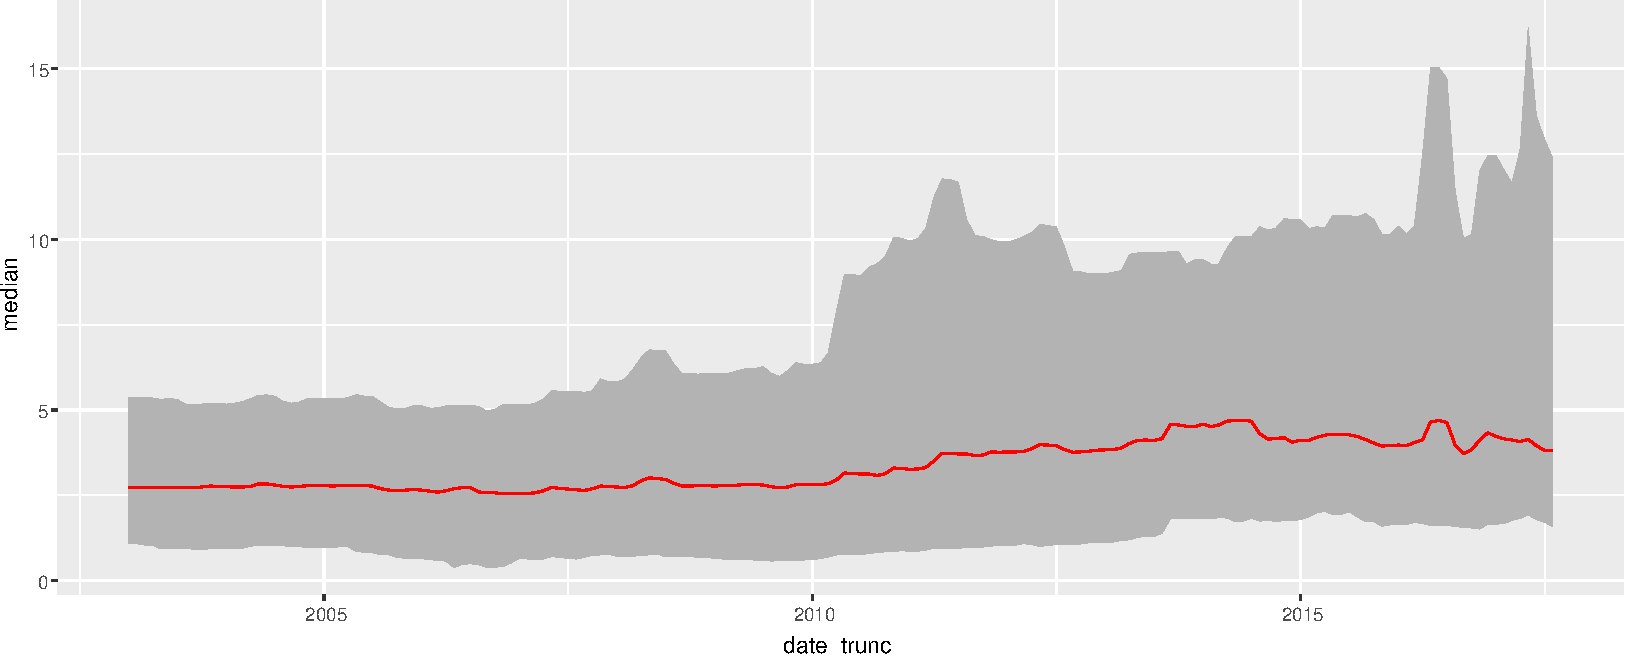
\includegraphics{PB-ROE_files/figure-latex/unnamed-chunk-4-1.pdf}
\caption{Bps全市场历史统计}
\end{figure}

近期,每股账面价格确实有下降的趋势,但是

\begin{itemize}
\tightlist
\item
  幅度不大
\item
  每股账目价格下降只是在最近出现的情况,在2010年时没有这样的现象。
\end{itemize}

公司账面价值的变化,依旧不能解释价格泡沫过后出现的PB``估值泡沫''的发生的原因\footnote{我们姑且把这一现象称之为“泡沫”。}。我们需要进一步的分析PB变化的原因。

\begin{figure}[htbp]
\centering
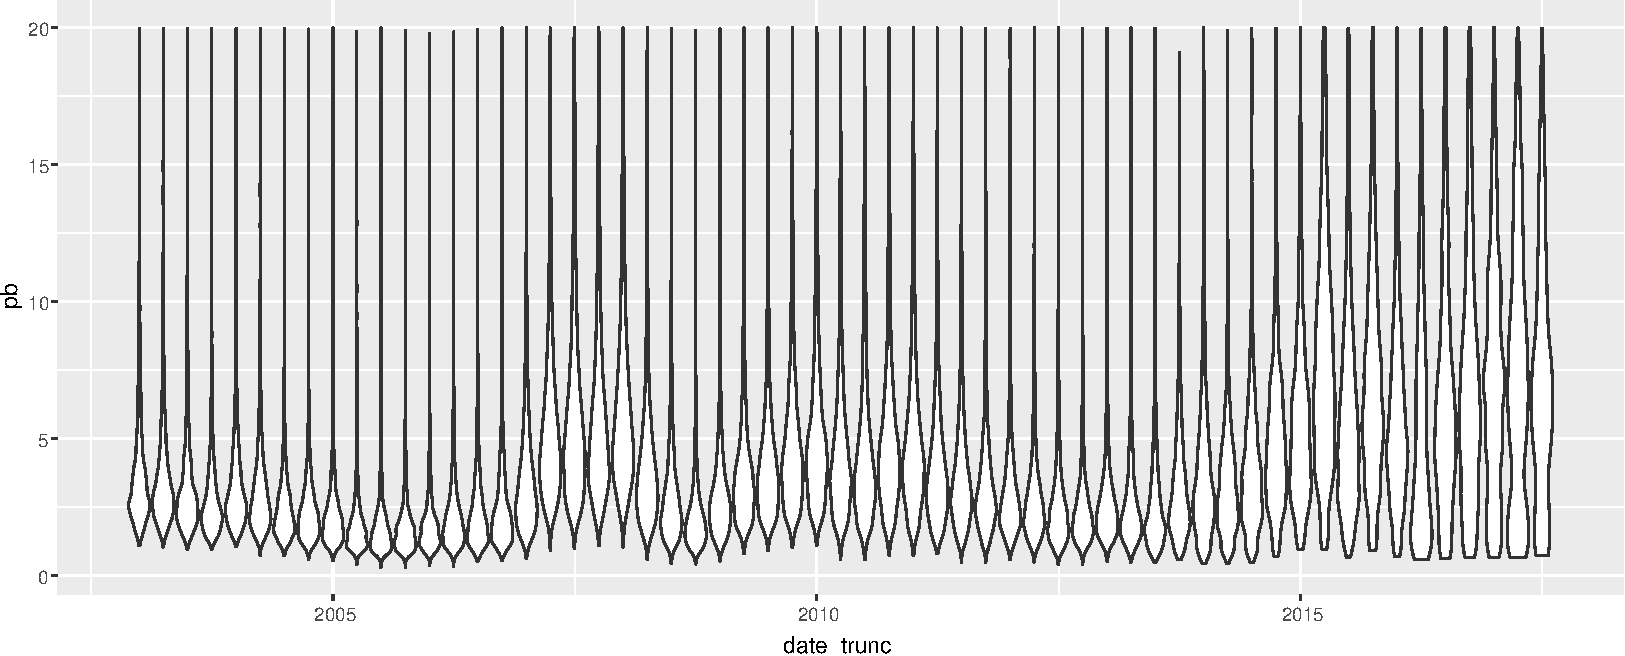
\includegraphics{PB-ROE_files/figure-latex/unnamed-chunk-5-1.pdf}
\caption{PB全市场历史分布}
\end{figure}

上图中,我们勾画了每个季度PB值分布的概率密度函数,从中可以看出2007年和2015年泡沫时期PB的分布是纺锤形的,2010年的``反弹''与当前的反弹在PB分布上是不同。2010年市场PB值的分布与2007年市场泡沫时候是类似的纺锤型,显示的是整体估值水平的上升,背后的动因是4万亿货币放水。当前市场反弹中的PB值的分布是类似哑铃型和沙袋型的,显示的是在市场恢复中部分股票的估值上升,而比部分股票依旧保持较低的估值水平。这体现出该时期不同类型股票估值风格上的变化,暗示的是一种市场结构上的变化。这是积极的一面,另一面是,毕竟整体上估值上升了,且估值水平不低,风险正在孕集。

\end{document}
